\documentclass[12pt, twoside]{book}
%\documentclass[12pt, oneside]{book}  % jednostranna tlac

%spravne nastavenie okrajov
\usepackage[a4paper,top=2.5cm,bottom=2.5cm,left=3.5cm,right=2cm]{geometry}
%zapnutie fontov pre UTF8 kodovanie
\usepackage[utf8]{inputenc}
\usepackage[T1]{fontenc}
\usepackage[inkscapeformat=png]{svg}
\usepackage{graphicx}		
\usepackage{amsmath,amsfonts,amssymb}
\usepackage{lipsum}
\usepackage{xcolor}
\usepackage{subcaption}
\DeclareMathOperator*{\argmin}{arg\,min}
\usepackage{listings}

%Code listing style named "mystyle"

%zapnutie slovenskeho delenia slov
%a automatickych nadpisov ako Obsah, Obrázok a pod. v slovencine
%\usepackage[slovak]{babel} % vypnite pre prace v anglictine!

%nastavenie riadkovania podla smernice
\linespread{1.25} % hodnota 1.25 by mala zodpovedat 1.5 riadkovaniu

% balicek na vkladanie zdrojoveho kodu
% ukazky kodu su cislovane ako Listing 1,2,...
% tu je Listing zmenene na Algoritmus 1,2,...
\renewcommand{\lstlistingname}{Algorithm}
% nastavenia balicka listings
% mozete pridat aj language=...
% na nastavenie najcastejsie pouzivaneho prog. jazyka
% takisto sa da zapnut cislovanie riadkov
\lstset{frame=lines}

% balicek na vkladanie obrazkov
\usepackage{graphicx}
% balicek na vkladanie celych pdf dokumentov, tu zadanie
\usepackage{pdfpages}
% balicek na spravne formatovanie URL
\usepackage{url}
% balicek na hyperlinky v ramci dokumentu
% zrusime farebne ramiky okolo liniek aby pdf
% vyzeralo rovnako ako tlacena verzia
\usepackage[hidelinks,breaklinks]{hyperref}
\usepackage{hhline}

% -------------------
% --- Definicia zakladnych pojmov
% --- Vyplnte podla vasho zadania, rok ma byt rok odovzdania
% -------------------
\def\mfrok{2024}
\def\mfnazov{Auxiliary self-organization based loss for Semi-supervised learning}
\def\mftyp{Diploma Thesis}
\def\mfautor{Bc. Sabína Samporová}
\def\mfskolitel{RNDr. Kristína Malinovská, PhD.}

%ak mate konzultanta, odkomentujte aj jeho meno na titulnom liste
\def\mfkonzultant{tit. Meno Priezvisko, tit. }  

\def\mfmiesto{Bratislava, \mfrok}

% študenti BIN a DAV odkomentujú príslušnú dvojicu riadkov
\def\mfodbor{Informatics}
\def\program{Applied Informatics}
% pre BIN:
%\def\mfodbor{Computer Science and Biology} 
%\def\program{ Bioinformatics }
% pre DAV:
%\def\mfodbor{Computer Science and Mathematics} 
%\def\program{ Data Science }

% Ak je školiteľ z FMFI, uvádzate katedru školiteľa, zrejme by mala byť aj na zadaní z AIS2
% Ak máte externého školiteľa, uvádzajte Katedru informatiky 
\def\mfpracovisko{ Department of Informatics}

\begin{document}     
\frontmatter
\pagestyle{empty}

% -------------------
% --- Obalka ------
% -------------------

\begin{center}
  \sc\large
  Comenius University in Bratislava\\
  Faculty of Mathematics, Physics and Informatics
\end{center}



\vfill

\begin{center}
\sc\large
{\LARGE\mfnazov}\\
\mftyp
\end{center}

\vfill

{\sc\large 
\noindent \mfrok\\
\mfautor
}

\cleardoublepage
% --- koniec obalky ----

% -------------------
% --- Titulný list
% -------------------

\noindent

\begin{center}
\sc  
\large
  Comenius University in Bratislava\\
  Faculty of Mathematics, Physics and Informatics
\end{center}

\vfill
\begin{figure}[h!]
    \centering
    
\includegraphics[width=0.5\textwidth]{figs/FMFI_logo_BP.png}
\end{figure}

\vfill


\begin{center}
{\LARGE\mfnazov}\\
\mftyp
\end{center}

\vfill

\noindent
\begin{tabular}{ll}
Study Programme: & \program \\
Field of Study: & \mfodbor \\
Department: & \mfpracovisko \\
Supervisor: & \mfskolitel \\
% Consultant: & \mfkonzultant \\
\end{tabular}

\vfill


\noindent \mfmiesto\\
\mfautor

\cleardoublepage
% --- Koniec titulnej strany


% -------------------
% --- Zadanie z AIS
% -------------------
% v tlačenej verzii s podpismi zainteresovaných osôb.
% v elektronickej verzii sa zverejňuje zadanie bez podpisov
% v pracach v anglictine anglicke aj slovenske zadanie

\newpage
\setcounter{page}{2}
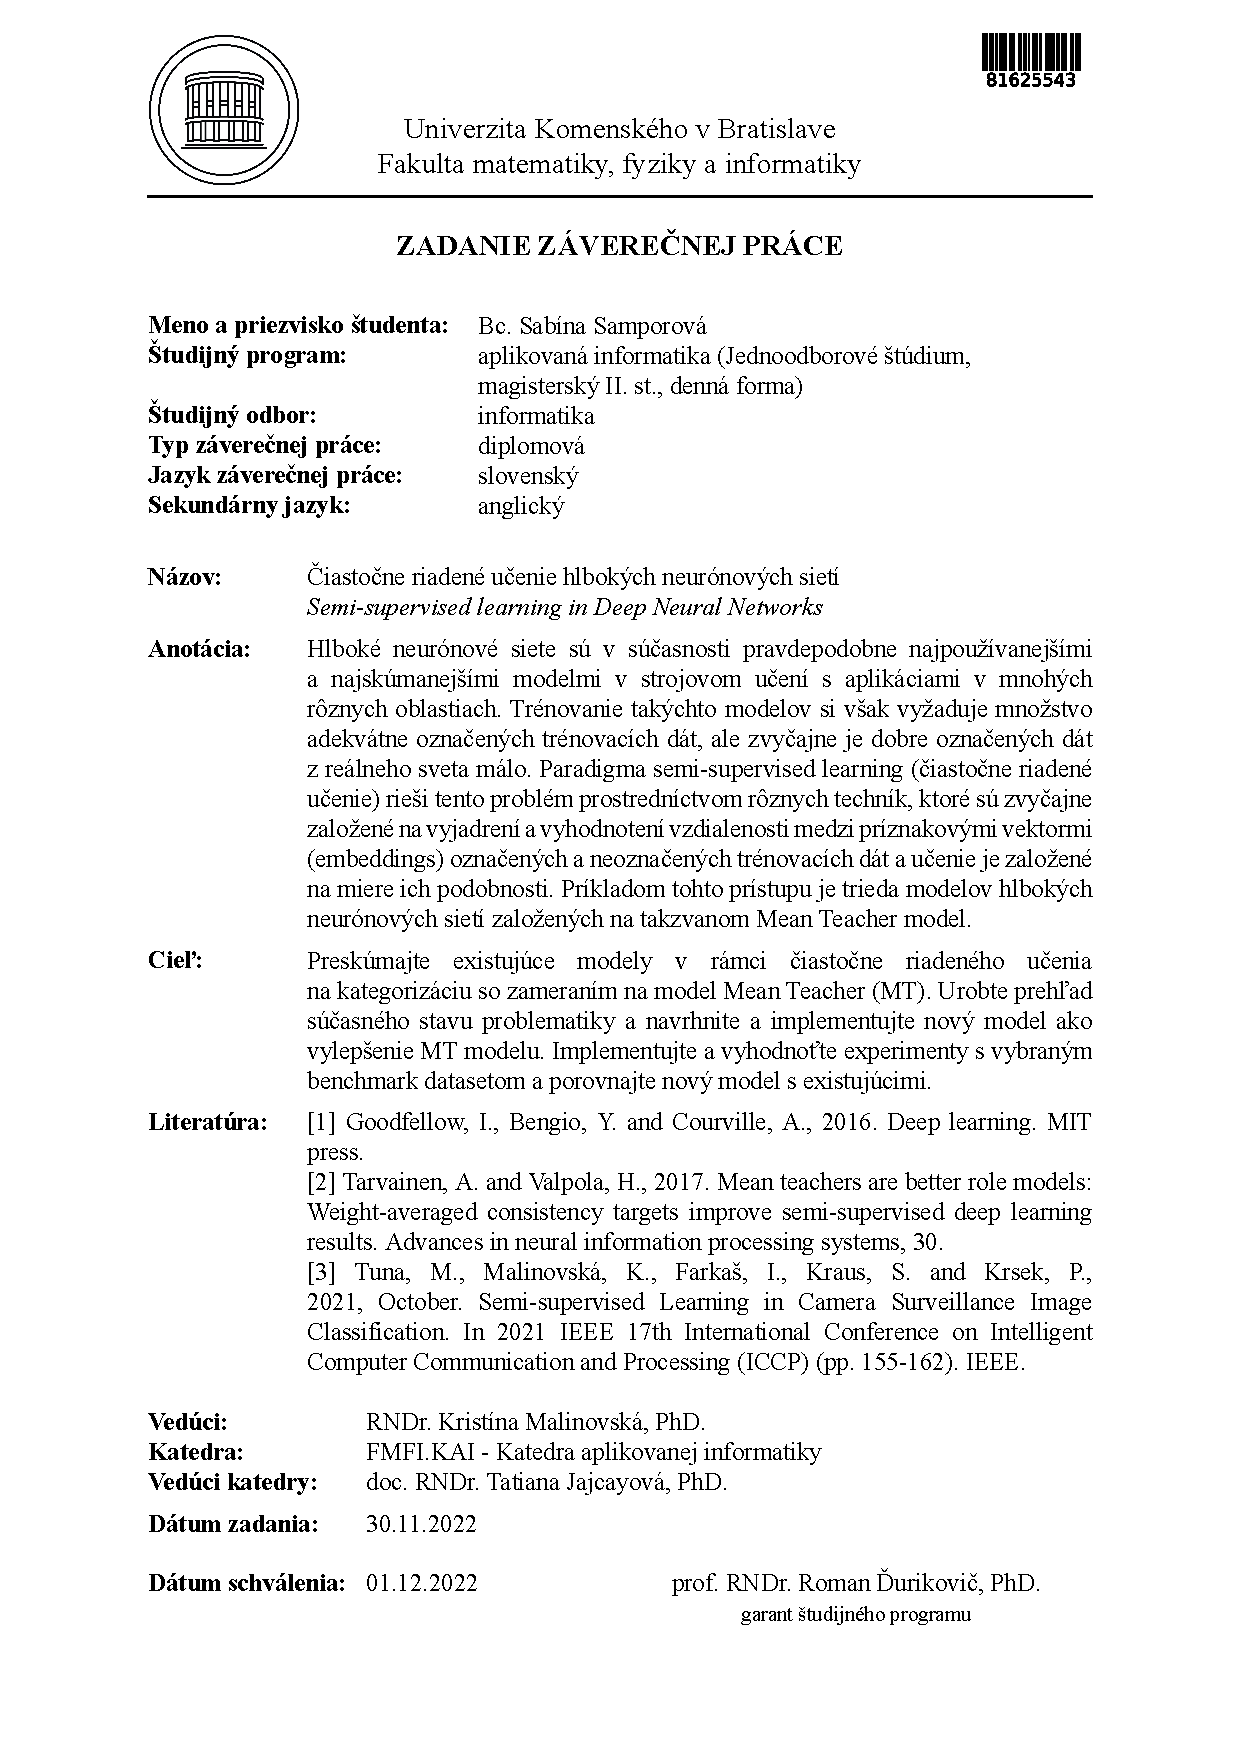
\includepdf{zadanie/zadanie.pdf}

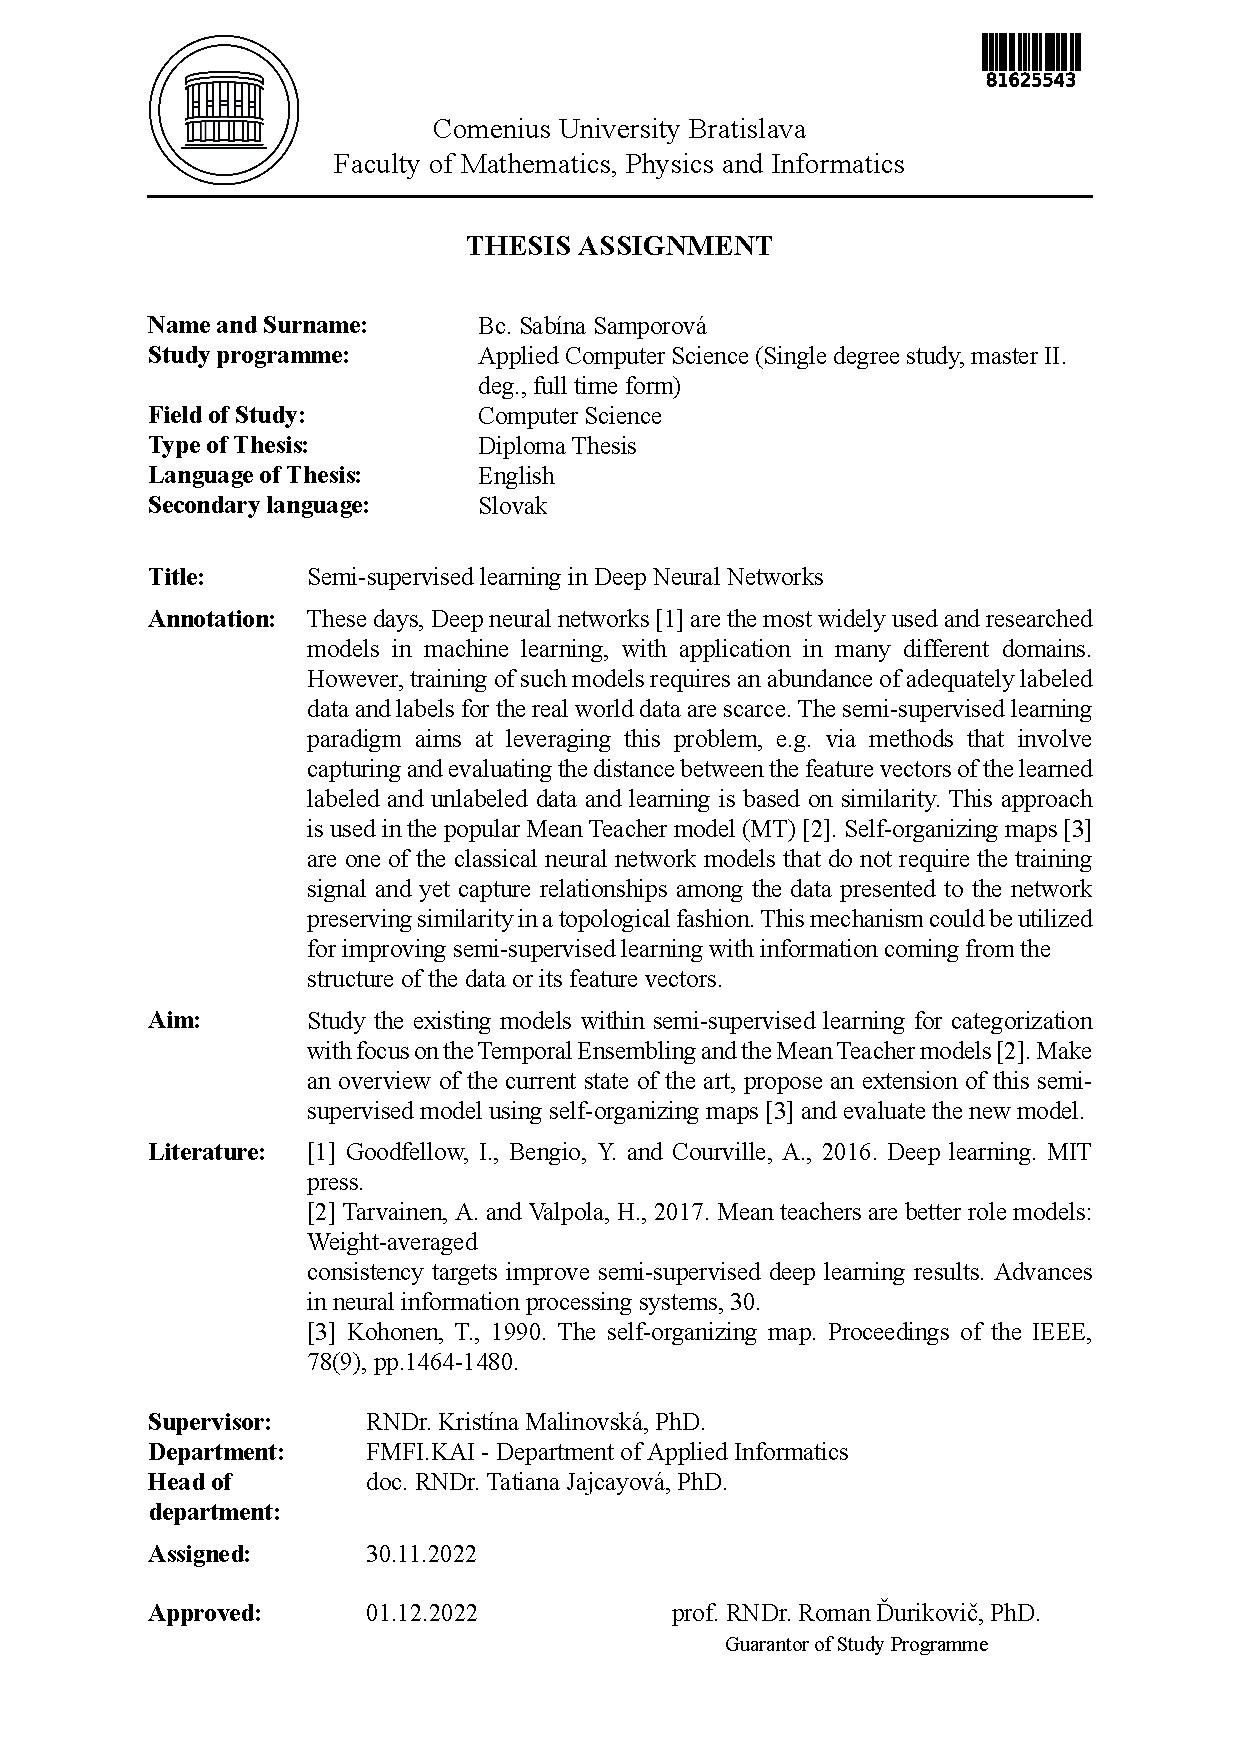
\includepdf{zadanie/zadanie-zp-en.pdf}

% --- Koniec zadania


% -------------------
%   Poďakovanie - nepovinné
% -------------------
\newpage
\pagestyle{plain}
~

\vfill
{\bf Acknowledgments:} % \color{red} TODO \color{black}


% --- Koniec poďakovania

% -------------------
%   Abstrakt - Slovensky
% -------------------
\newpage 
\section*{Abstrakt}

Paradigma čiastočne riadeného učenia je alternatívou k najrozšírenejšiemu spôsou učenia umelých neurónových sietí - učeniu s učiteľom, ktoré na trénovanie modelu potrebuje súbor vstupných dát, z ktorého každý má priradené označenie. Neurónové siete, ktoré sú trénované pomocou čiastočne riadeného učenia, si vystačia s malou časťou označených dát a väčším množstvom neoznačených dát. Keďže priradzovanie označní k údajom je náročné na zdroje, táto paradigma môže časovo zefektívniť prípravu modelu.
V tejto diplomovej práci sme navrhli model MT-SOM, rozšírenie čiastočne riadeného modelu Mean teacher, vylepšené o samoorganizáciu. Samoorganizácia je zapojená prostredníctvom stratovej funkcie, ktorú sme tiež navrhli. Ukázali sme, že tento model má lepšiu testovaciu presnosť ako základný model trénovaný s učiteľom, s rovnakým podielom označených dát a vďaka tomu môže byť užitočný pre úlohy v čiastočne-riadenom nastavení. Počas vývoja modelu MLP-SOM sme testovali stratovú funkciu založenú na samoorganizácii aj v učení s učiteľom a ukázali sme, že aj v tejto situácii pomocná stratová funkcia pomáha výkonu modelu.



\paragraph*{Kľúčové slová:} umelé neurónové siete, čiastočne riadené učenie, Mean teacher model, samoorganizácia, Samo-organizujúca sa mapa, pomocná stratová funkcia


% --- Koniec Abstrakt - Slovensky


% -------------------
% --- Abstrakt - Anglicky 
% -------------------
\newpage 
\section*{Abstract}

Semi-supervised learning paradigm is alternative to most used supervised learning, which need labeled dataset for model training. Neural networks that are trained in semi-supervised setup suffice with small portion of labeled data and greater amount of unlabeled data. Since labeling the data is demanding on resources, this paradigm can make model training more time-efficient.
In this thesis, we proposed MT-SOM model, extension of Mean teacher semi-supervised model, which improve semi-supervised model with self-organization. The self-organization is engaged via loss function, which we also proposed. We shown, that this model has better performance, that supervised baseline with the same portion of labeled samples, therefore it can be useful for semi-supervised tasks. During development of MLP-SOM model, we tested self-organization based loss also in supervised task and showed that also in supervised setup, auxiliary loss helped performance of the model.


\paragraph*{Keywords:} artificial neural networks, semi-supervised learning, Mean teacher model, self-organization, Self-organizing map, auxiliary loss


% --- Koniec Abstrakt - Anglicky

% -------------------
% --- Predhovor - v informatike sa zvacsa nepouziva
% -------------------
%\newpage 
%
%
%\chapter*{Preface} %
%
%Predhovor je všeobecná informácia o práci, obsahuje hlavnú charakteristiku práce 
%a okolnosti jej vzniku. Autor zdôvodní výber témy, stručne informuje o cieľoch 
%a význame práce, spomenie domáci a zahraničný kontext, komu je práca určená, 
%použité metódy, stav poznania; autor stručne charakterizuje svoj prístup a svoje
%hľadisko. 
%
% --- Koniec Predhovor


% -------------------
% --- Obsah
% -------------------

\newpage 

\tableofcontents

% ---  Koniec Obsahu

% -------------------
% --- Zoznamy tabuliek, obrázkov - nepovinne
% -------------------

\newpage 

\listoffigures
\listoftables

% ---  Koniec Zoznamov

\mainmatter
\pagestyle{headings}

\input 0-intro.tex 

\input 1-overview.tex

\input 2-bmt-exp.tex

\input 3-proposition.tex

\input 4-som-loss.tex

\input 5-som-fv-cifar.tex

\input 6-research-results.tex

\input 7-conclusion.tex

%\input kapitola.tex

%\input latex.tex



%\input zaver.tex

% -------------------
% --- Bibliografia
% -------------------


\newpage	

\backmatter

\thispagestyle{empty}
\clearpage

\bibliographystyle{plain}
\bibliography{literatura} 

%Prípadne môžete napísať literatúru priamo tu
%\begin{thebibliography}{5}
 
%\bibitem{br1} MOLINA H. G. - ULLMAN J. D. - WIDOM J., 2002, Database Systems, Upper Saddle River : Prentice-Hall, 2002, 1119 s., Pearson International edition, 0-13-098043-9

%\bibitem{br2} MOLINA H. G. - ULLMAN J. D. - WIDOM J., 2000 , Databasse System implementation, New Jersey : Prentice-Hall, 2000, 653s., ???

%\bibitem{br3} ULLMAN J. D. - WIDOM J., 1997, A First Course in Database Systems, New Jersey : Prentice-Hall, 1997, 470s., 

%\bibitem{br4} PREFUSE, 2007, The Prefuse visualization toolkit,  [online] Dostupné na internete: <http://prefuse.org/>

%\bibitem{br5} PREFUSE Forum, Sourceforge - Prefuse Forum,  [online] Dostupné na internete: <http://sourceforge.net/projects/prefuse/>

%\end{thebibliography}

%---koniec Referencii

% -------------------
%--- Prilohy---
% -------------------

%Nepovinná časť prílohy obsahuje materiály, ktoré neboli zaradené priamo  do textu. Každá príloha sa začína na novej strane.
%Zoznam príloh je súčasťou obsahu.
%
%\input appendixA.tex

%\input appendixB.tex

\end{document}






